\section{Analyse des résulats}
\subsection{Un premier résultat préliminaire}
On teste l'algorithme de descente de gradient pour un nombre d'onde $k=1$ et un mur de fractale de niveau 2.
La Figure \ref{fig:ene1} représente l'évolution de l'énergie (ou la fonction coût) en fonction du nombre d'itérations lors de l'application de l'algorithme d'optimisation par descente de gradient. Le nouveau $\chi$ calculé par l'algorithme permet de diminuer l'énergie au sein du réacteur.

\begin{figure}[H]
    \centering
    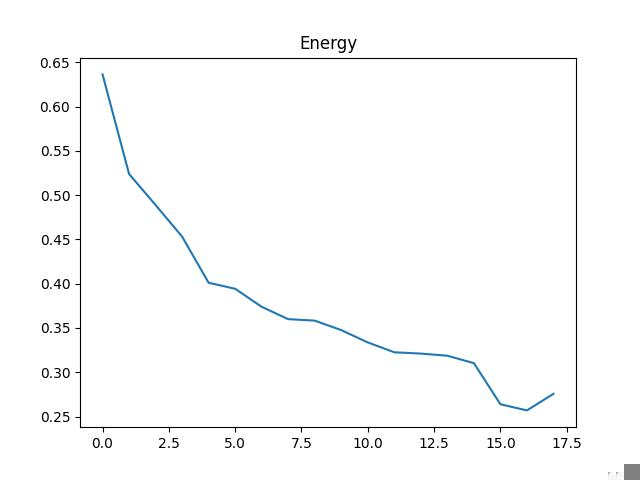
\includegraphics[width=0.5\linewidth]{rapport//numerique//exemplek1/k0descgradenergy.jpg}
    \caption{Énergie en fonction du nombre d'itération}
    \label{fig:ene1}
\end{figure}



\begin{figure}[H]
    \centering
    \subfloat{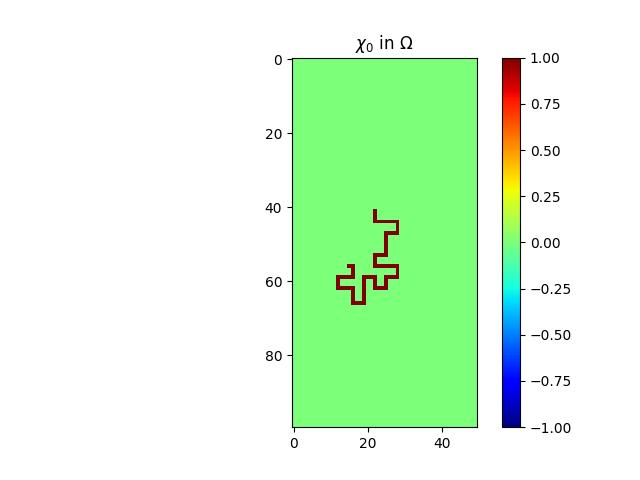
\includegraphics[width = 3.0in]{rapport/numerique/exemplek1/fig_chi0_re_plot_k1.jpg}
    \subfloat{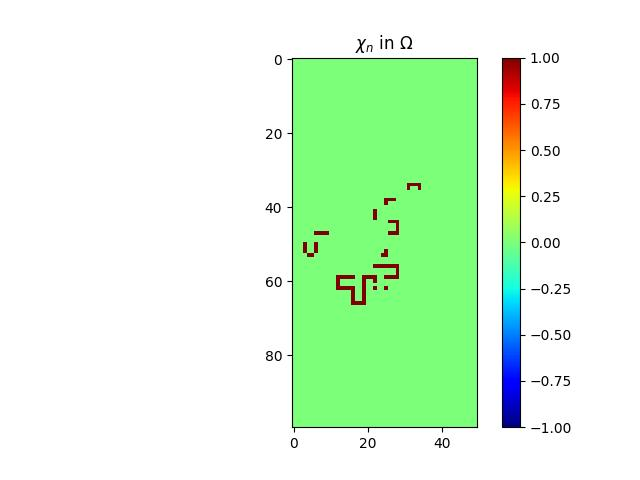
\includegraphics[width = 3.0in]{rapport/numerique/exemplek1/fig_chin_re_plot_k1.jpg}}\\
    \caption{$\chi$ avant et après optimisation et projection}
    \label{loca}
\end{figure}

\begin{figure}[H]
    \centering
    \subfloat{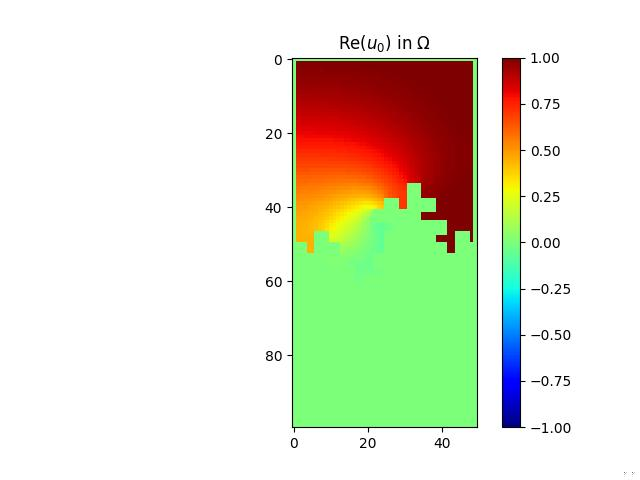
\includegraphics[width = 3.0in]{rapport/numerique/exemplek1/fig_u0_re_plot.jpg}}
    \subfloat{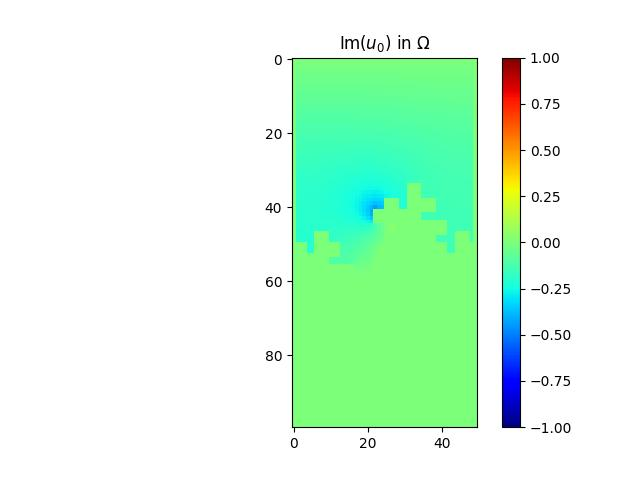
\includegraphics[width = 3.0in]{rapport/numerique/exemplek1/fig_u0_im_plot.jpg}}\\
    \caption{Solution $u$ avant optimisation}
    \label{loca}
\end{figure}

\begin{figure}[H]
    \centering
    \subfloat{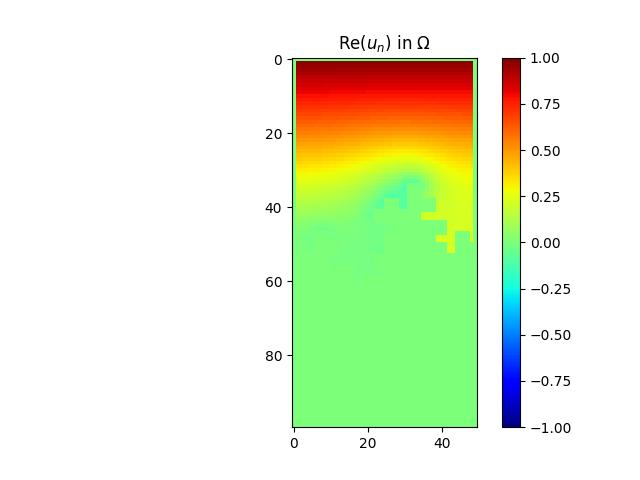
\includegraphics[width = 3.0in]{rapport/numerique/exemplek1/fig_un_re_plot.jpg}}
    \subfloat{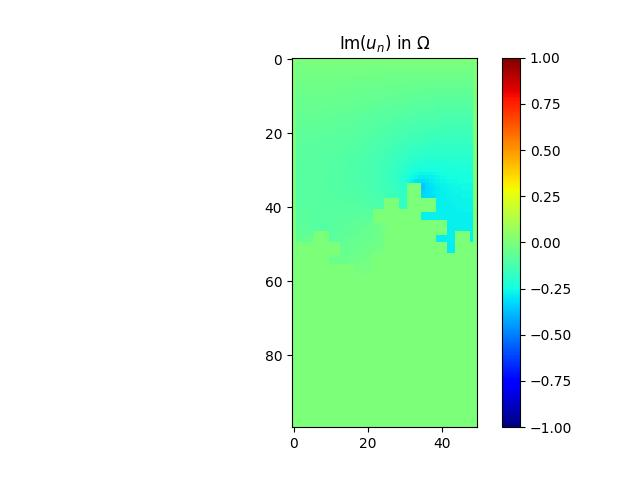
\includegraphics[width = 3.0in]{rapport/numerique/exemplek1/fig_un_im_plot.jpg}}\\
    \caption{Solution $u$ après optimisation}
    \label{loca}
\end{figure}


\subsection{Étude des bruits}
Pour que l'atténuation du bruit de l'avion soit efficace, il est nécessaire d'étudier la fréquence des bruits qui dérangent le plus. Les bruits crées par les moteurs d'avion proviennent de trois sources principalement: le ventilateur, la turbine et la combustion. La combinaison de ces bruits se situe généralement entre 100 Hz et 6 000 Hz. Étant donné que $ k = \omega/c = 2\pi f/c$, nous allons donc étudier le problème pour $k \in [1.85\,m^{-1}, 112\,m^{-1}].$ 

\subsection{Étude des matériaux}
Dans cette section, on fera une étude comparative entre différents matériaux qui peuvent être utilisés dans la fabrication des liners en termes de qualité d'absorption de l'énergie sonore que nous cherchons à minimiser. En effet, la qualité d'absorption du matériau dépend du coefficient $\alpha$ qui dépend lui même aussi de la fréquence utilisée. Comme il est nécessaire d'utiliser un matériau léger, résistant et poreux, nous avons choisi de comparer trois matériaux: l'Isorel, l'IFTH, et le mat q3. Ces matériaux ont 3 grandeurs caractéristiques qui affectent leur capacité d'absorbance, à savoir la porosité $\phi$, la résistivité $\sigma$ et la tortuosité $\alpha_{h}$, montrés dans le tableau suivant.
\begin{table}[H]
\centering
\begin{tabular}{|c|c|c|c|c|}
\hline
Caractéristique & mat q3 & IFTH  & Isorel \\ \hline
$\phi$ & 0.99 & 0.94 & 0.70 \\ \hline
$\sigma$ & 14000 & 9067 & 142300 \\ \hline
$\alpha_{h}$ & 1.02 & 1 & 1.15 \\ \hline
\end{tabular}
\caption{Caractéristiques des différentes matériaux}
\end{table}
Nous avons donc évalué le coefficient $\alpha$ de ces différents matériaux sur une plage de fréquences entre 50Hz et 1kHz. Les résultats de simulation sont les suivants.

\begin{figure}[H]
    \centering

    \subfloat{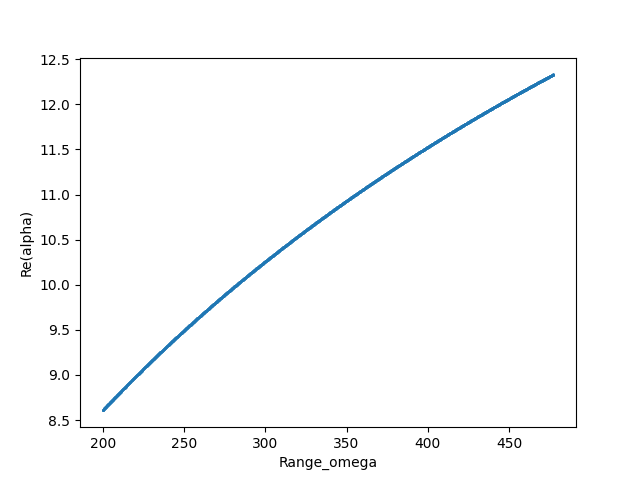
\includegraphics[width = 3.0in]{rapport/numerique/Re(alpha) mat q3.png}
    \subfloat{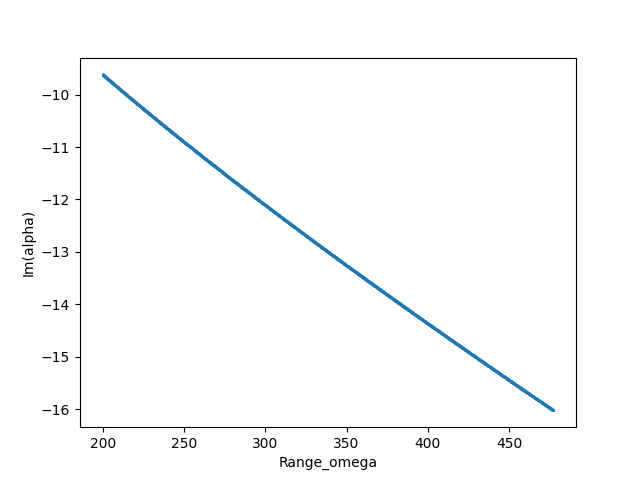
\includegraphics[width = 3.0in]{rapport/numerique/Im(alpha) mat q3.png}}\\
    \caption{$Re(\alpha)$ et $Im(\alpha)$ pour mat q3}
    \label{freq}
\end{figure}

\begin{figure}[H]
    \centering

    \subfloat{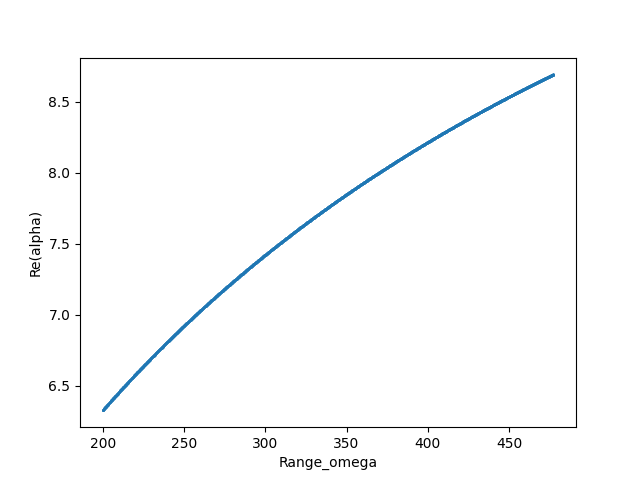
\includegraphics[width = 3.0in]{rapport/numerique/Re(alpha) ITFH.png}
    \subfloat{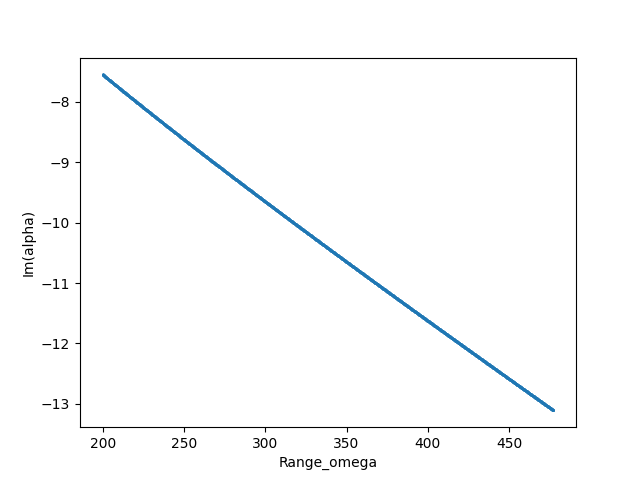
\includegraphics[width = 3.0in]{rapport/numerique/Im(alpha) ITFH.png}}\\
    \caption{$Re(\alpha)$ et $Im(\alpha)$ pour ITFH}
    \label{freq}
\end{figure}

\begin{figure}[H]
    \centering

    \subfloat{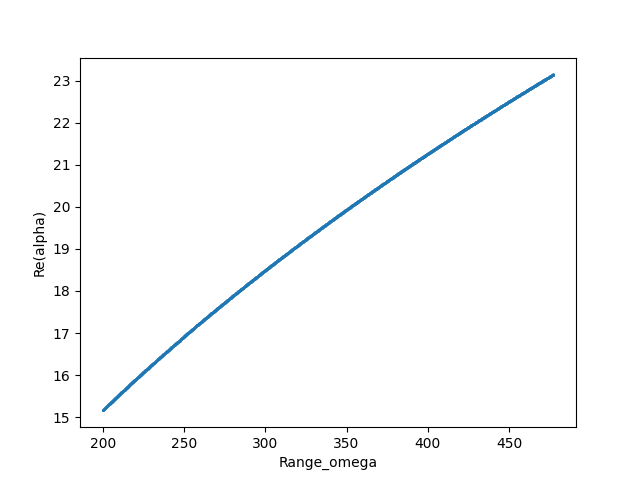
\includegraphics[width = 3.0in]{rapport/numerique/Re(alpha) isorel.png}
    \subfloat{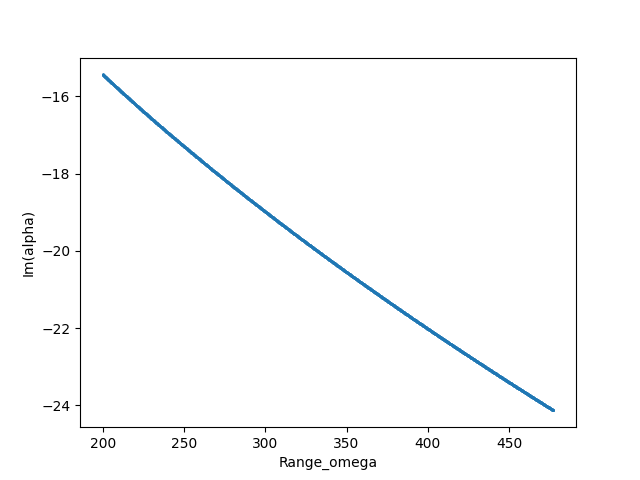
\includegraphics[width = 3.0in]{rapport/numerique/Im(alpha) ISOREL.png}}\\
    \caption{$Re(\alpha)$ et $Im(\alpha)$ pour ISOREL}
    \label{freq}
\end{figure}

La compréhension des courbes passe par l'évolution de la partie réelle et imaginaire de $\alpha$. En effet, plus le rapport de $\displaystyle \frac{Re(\alpha)}{Im(\alpha)}$
est proche de 0 plus le matériau est absorbant.
\begin{figure}[H]
    \centering
    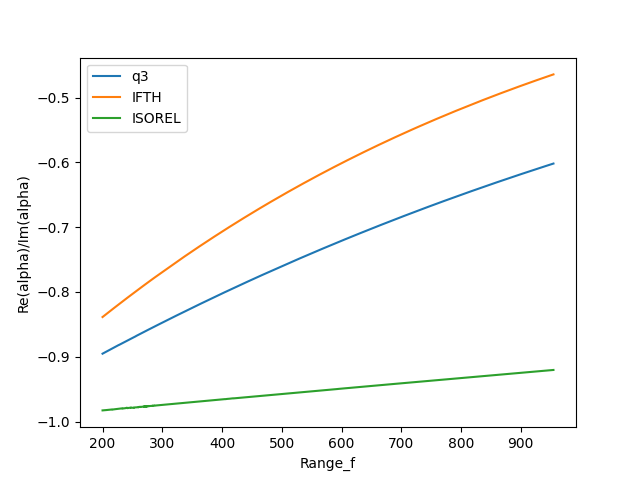
\includegraphics[width=0.5\linewidth]{rapport/numerique/Re(alpha) over Im(alpha)_ISOREL.png}
    \caption{$\displaystyle \frac{Re(\alpha)}{Im(\alpha)}$ pour les 3 matériaux}
    \label{fig:ene}
\end{figure}

La figure nous montre que c'est l'IFTH le matériau le plus absorbant parmi les 3 et c'est celui qu'il faut adopter pour la construction du matériau poreux au niveau de la frontière de bas.\\
Cependant, pour les sections qui suivent, nous utiliserons un coefficient $\alpha$ de $10-10j$ assez souvent afin de s'approcher de l'ordre de grandeur général des parties réelles et imaginaires de $\alpha$ trouvées pour les différents matériaux étudiés.

\subsection{Étude de la géométrie}
Dans cette section, nous étudions l'énergie au sein du réacteur en fonction de la géométrie de la frontière afin de déterminer la géométrie la plus efficace. Pour cette étude, la frontière est totalement absorbante (\textit{id est} \\ $V = \displaystyle \frac{\int_{\Gamma_{abs}} \chi dS}{\int_{\Gamma_{abs}} dS} = 1$), et on trace l'énergie sur toute la gamme de fréquence considérée pour chaque niveau de fractale.
\begin{figure}[H]
    \centering
    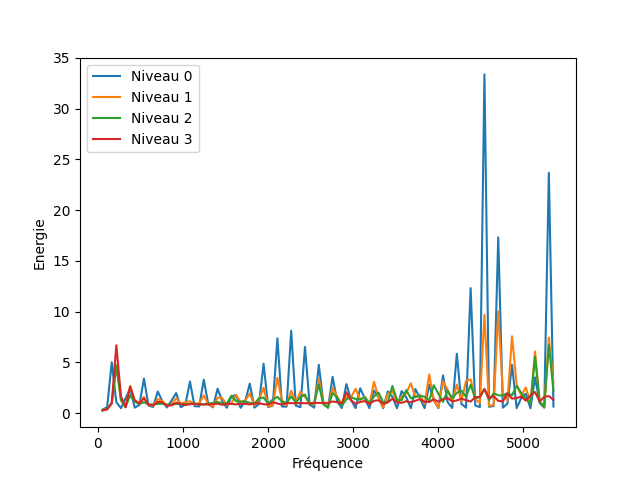
\includegraphics[width=0.5\linewidth]{rapport/numerique/exemplek1/fullabs.png}
    \caption{Frontière totalement absorbante pour différents niveaux de fractale}
    \label{fig:enter-label}
\end{figure}
Nous obtenons le tableau suivant.
\begin{table}[H]
    \centering
    \begin{tabular}{ccc}
        Fractale & Énergie Max  & Énergie Moyenne\\
         Niveau 0& 33,4 & 2,45 & \\
         Niveau 1 & 10,0 & 1,88 & \\
         Niveau 2 & 6,74 & 1,51 & \\
         Niveau 3 & 6,70 & 1,20 & \\
    \end{tabular}
    \label{tab:my_label}
\end{table}
Ainsi une fractale de niveau 2 et de niveau 3 atténue bien mieux les bruits. Dans la suite de l'étude, nous ne considérons seulement ces deux niveaux de fractale.\\ \\
Cependant, une remarque doit être vis-à-vis des différents niveaux de fractale choisis. Plus le niveau de fractale est élevé, plus la longueur de la paroi est grande et plus la quantité de matériaux nécessaire augmente. Le choix de conserver les niveaux 2 et 3 seulement s'explique par le fait que nous voulons une solution de bonne qualité, même si cela nécessite plus de matériaux. Néanmoins, il se peut que nous privilégions le niveau 2 au 3 car le niveau 3 n'apporte pas suffisamment de réduction par rapport au niveau 2.

\subsection{Étude de la quantité de matériaux}
On étudie l'efficacité de l'atténuation en fonction de la quantité de matériaux utilisé par le liner afin de trouver le meilleur compromis entre atténuation et coût.
    \begin{figure}[H]
    \centering
    \subfloat{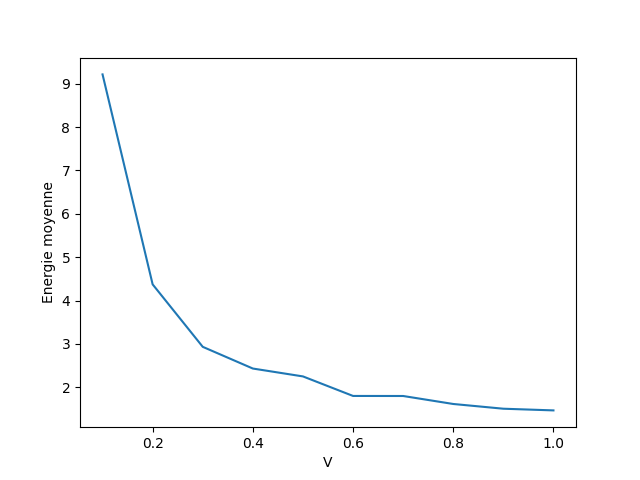
\includegraphics[width = 3.0in]{rapport/numerique/exemplek1/lvl2.png}}
    \subfloat{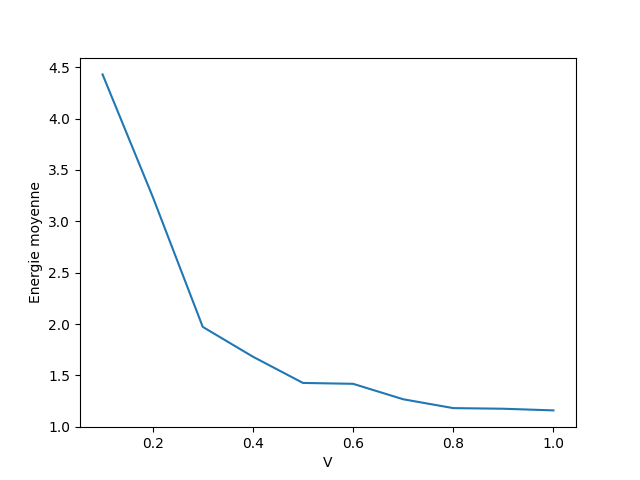
\includegraphics[width = 3.0in]{rapport/numerique/assets/lvl3.png}}\\
    \caption{Énergie moyenne après optimisation en fonction de $V$ pour la fractale de niveau 2 (gauche) et 3 (droite)}
    \label{freq}
\end{figure}

\subsection{Optimisation mono-fréquentielle}

Dans cette section, nous allons optimiser la disposition du liner pour atténuer les fréquences les plus problématiques. Pour chaque niveau de fractale, on choisit les 7 fréquences pour lesquelles les énergies sont les plus grandes. La Figure \ref{freq1} montre que pour toutes ces fréquences problématiques, l'énergie après optimisation diminue largement. Notre algorithme permet donc d'atténuer les fréquences problématiques.

\begin{figure}[H]
    \centering
    \subfloat{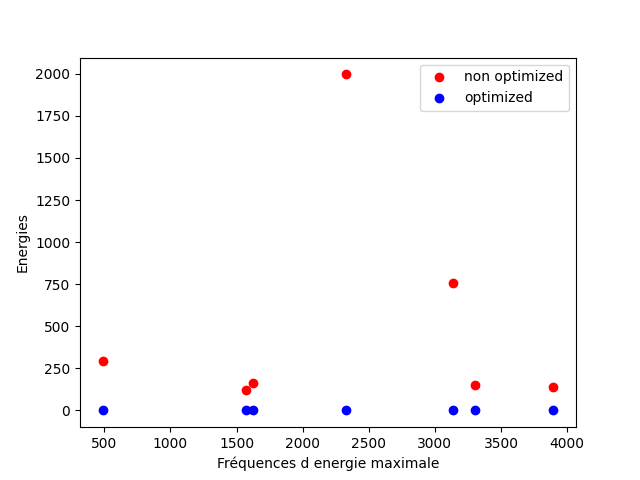
\includegraphics[width = 3.0in]{rapport/numerique/assets/Level_2_Alpha_absorp_N_50.png}}
    \subfloat{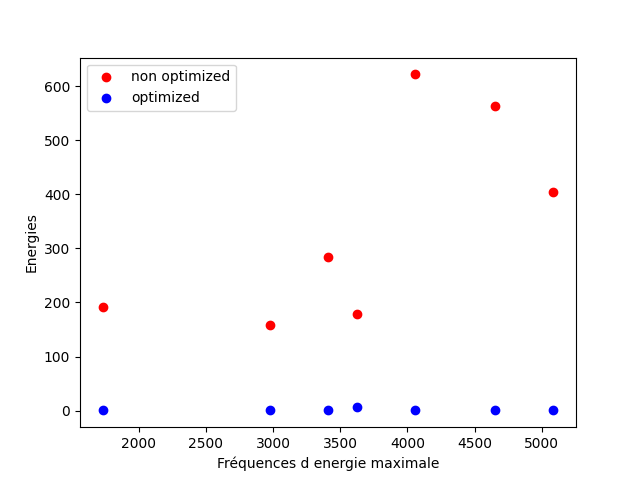
\includegraphics[width = 3.0in]{rapport/numerique/assets/Level_3_Alpha_absorp_N_50.png}}\\
    \caption{Les énergies maximales en fonction de la fréquence pour une fractale de niveau 2 et 3}
    \label{freq1}
\end{figure}

\subsection{Optimisation multi-fréquentielle}
La section précédente montre que notre algorithme est efficace pour chacune des fréquences considérées comme problématique, nous cherchons maintenant à étudier s'il est possible d'optimiser pour l'ensemble de ces fréquences simultanément. Nous devons alors adapter notre algorithme de descente de gradient. 

En effet, la nouvelle fonction de coût à considérer est la somme des énergies des fréquences pour un même $\chi$ pondérées avec des réels $(\lambda_{k})_{k \in K}$ (nous avons pris l'énergie avant: \textcolor{blue}{$$J(\chi) := \sum_{k} \lambda_{k} \int_\Omega |p_{k_{\chi}}|^2$$} et le gradient à considérer est alors la somme des gradients de chaque fréquence pondérée : \textcolor{blue}{$$J'(\chi) := - \sum_{k} \lambda_{k} \text{Re}(\alpha p_{k} q_{k}).$$}

En cherchant à minimiser la fonction de coût, l'algorithme va donner $\chi $ qui minimise globalement pour l'ensemble des fréquences considérées. Pour le choix des coefficients de pondération $\lambda_{k}$, nous avons pris l'énergie pour une onde de nombre de d'onde $k$ avant optimisation. 
Cependant, ce nouveau algorithme effectue beaucoup plus de calcul, c'est pourquoi nous nous limitons aux dix premiers $k$ en énergie pour avoir un temps de calcul raisonnable. Nous avons aussi limiter un nombre d'itération maximale à 10.

\begin{figure}[H]
    \centering
    \subfloat{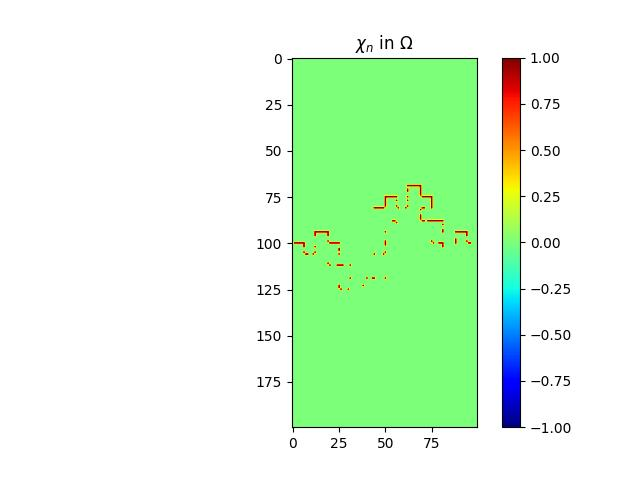
\includegraphics[width = 3.0in]{rapport/numerique/exemplek1/chimulti2.jpg}}
    \subfloat{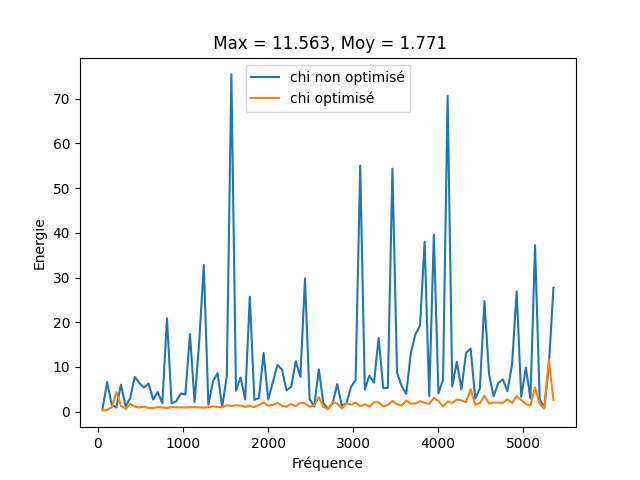
\includegraphics[width = 3.0in]{rapport/numerique/exemplek1/multi2.png}}\\
    \caption{Optimisation multi-fréquentielle avec fractale de niveau 2}
    \label{freq}
\end{figure}
\begin{figure}[H]
    \centering
    \subfloat{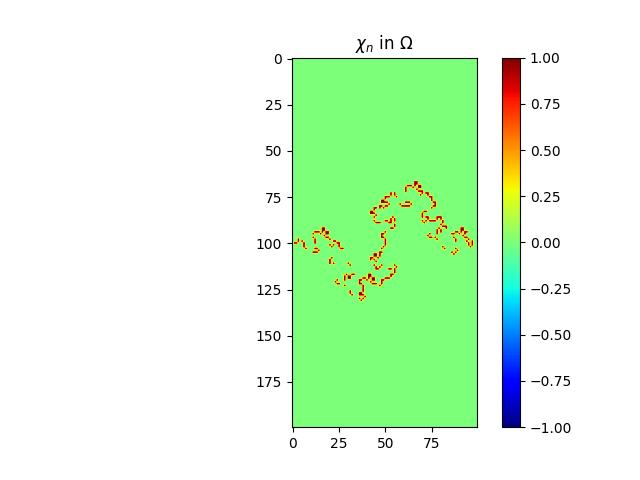
\includegraphics[width = 3.0in]{rapport/numerique/exemplek1/chimulti3.jpg}
    \subfloat{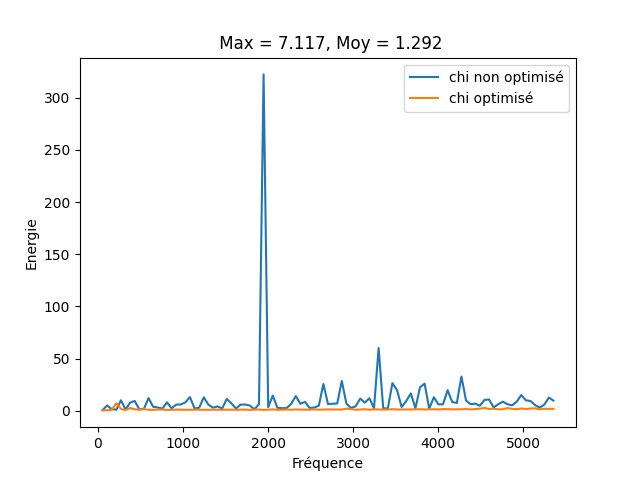
\includegraphics[width = 3.0in]{rapport/numerique/exemplek1/multi3.png}}\\
    \caption{Optimisation multi-fréquentielle avec fractale de niveau 3}
    \label{freq}
\end{figure}
Les figures obtenues montrent que l'optimisation multi-fréquentielle est très efficace: après optimisation, pour les niveaux de fractale, l'énergie est relativement faible sur toute la gamme de fréquence.

\subsection{Autre approche : optimisation stochastique}
On se propose d'étudier ce problème d'optimisation en utilisant une autre méthode que l'algorithme de descente gradient, plus particulièrement l'algorithme d'optimisation stochastique Hill Climbing. On commence par générer $\chi$ aléatoirement. A chaque itération, on explore le voisinage de $\chi$ en ajoutant un bruit blanc à $\chi$. Si avec le $\chi$ bruité l'énergie diminue, alors l'ancien $\chi$ est remplacé par le $\chi$ bruité, puis on itère un certain nombre de fois.
Expérimentalement on observe qu'entre le début et la fin de l'algorithme, la différence d'énergie est minimale. C'est pourquoi on limite à une seule itération, ce qui revient à utiliser un $\chi$ aléatoire.

\begin{figure}[H]
    \centering
    \subfloat{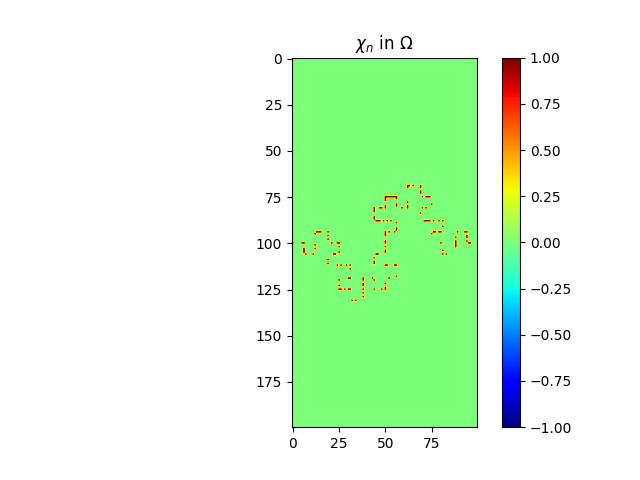
\includegraphics[width = 3.0in]{rapport/numerique/assets/rand/chi_rand_2.jpg}}
    \subfloat{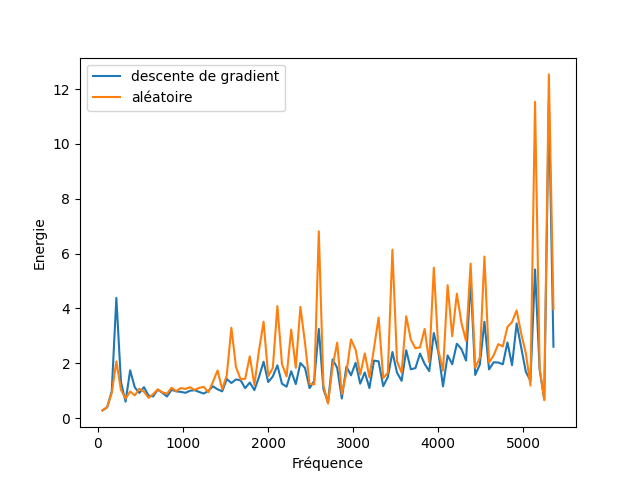
\includegraphics[width = 3.0in]{rapport/numerique/exemplek1/vslvl2.png}}\\
    \caption{Optimisation stochastique avec fractale de niveau 2}
    \label{vs1}
\end{figure}
\begin{figure}[H]
    \centering
    \subfloat{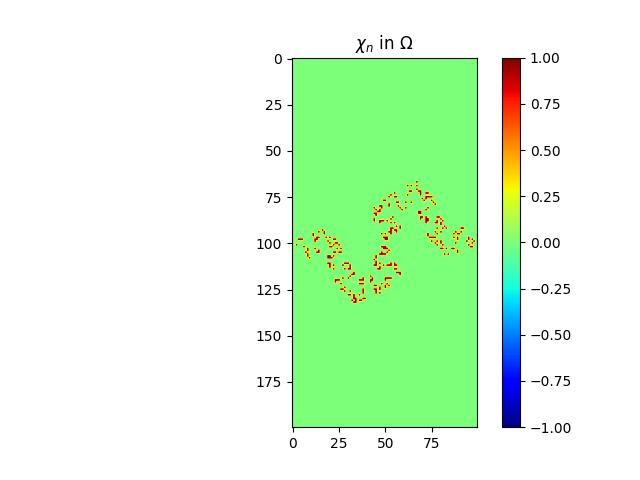
\includegraphics[width = 3.0in]{rapport/numerique/exemplek1/chi_rand_3.jpg}
    \subfloat{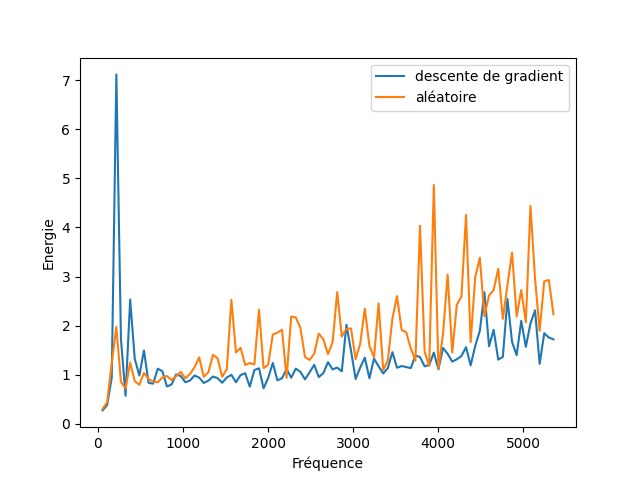
\includegraphics[width = 3.0in]{rapport/numerique/exemplek1/vslvl3.png}}\\
    \caption{Optimisation stochastique avec fractale de niveau 3}
    \label{vs2}
\end{figure}

D'après les Figures \ref{vs1} et \ref{vs2}, on conclut que l'optimisation stochastique est légèrement moins efficace que l'algorithme de descente de gradient multi-fréquentielle. Cependant, elle est également beaucoup plus rapide à calculer. De plus, on peut remarquer que pour la fractale de niveau 3, pour une fréquence particulière, l'énergie de la solution donnée par l'algorithme de descente de gradient est bien plus élevée que celle du $\chi$ aléatoire. \\ \\
Le caractère aléatoire de cette méthode d'optimisation va permettre d'avoir un $\chi$ qui est généralement réparti plutôt uniformément sur toute la paroi du réacteur, d'où l'atténuation efficace.

\subsection{Solution retenue}

D'après l'ensemble des études effectuées, la solution retenue est une fractale de niveau 2, $V = 0,5$, optimisé avec l'algorithme de descente de gradient multi-fréquentielle. On peut comparer son efficacité avec une fractale de niveau 3 entièrement absorbant dans la Figure \ref{abs22}.
\begin{figure}[H]
    \centering
    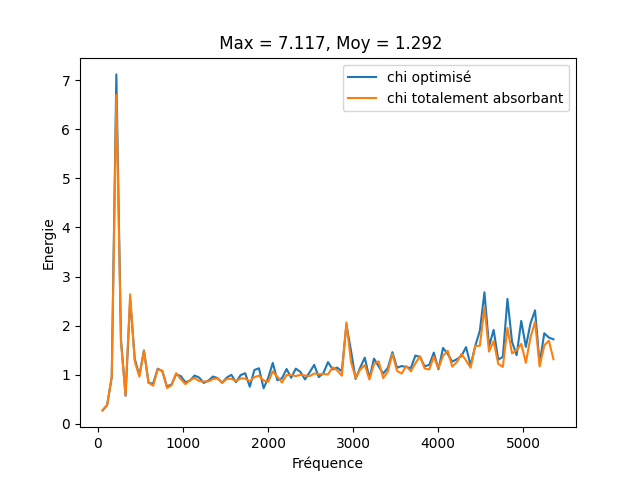
\includegraphics[width=0.5\linewidth]{rapport/numerique/exemplek1/solvsfullabs.png}
    \caption{Comparaison entre notre solution optimisée et $\chi$ totalement absorbant}
    \label{abs22}
\end{figure}
On peut remarquer la performance de la solution optimisée est très proche de $\chi$ totalement absorbant, voire meilleure pour certaines fréquences, alors qu'on utilise beaucoup moins de matériau absorbant ! 

\subsection{Conclusion de la partie numérique}
En résumé, notre démarche pour résoudre le problème posé est la suivante :
    \begin{itemize}
        \item Implémentation d'un algorithme de descente de gradient;
        \item Plusieurs études pour choisir des paramètres adaptés;
        \item Détermination de la meilleure solution en tenant en compte des études précédentes.
    \end{itemize}
Nous envisageons également quelques pistes d'amélioration possibles: 
    \begin{itemize}
        \item Meilleur ajustement des hyperparamètres (comme le learning rate) ;
        \item Mise à jour dynamique des coefficients de pondération pendant l'algorithme de descente de gradient multi-fréquentielle. En effet, les fréquences problématiques peuvent changer lorsque $\chi$ est modifié ;
        \item Calculer la réduction de bruit réelle en décibel ;
        \item Explorer d'autres algorithmes d'optimisation, comme l'algorithme génétique par exemple.
    \end{itemize}
\end{frame}